\section{Database design description}
{\it Note the difference between 'main user' and 'user'. Main user refers to the 
user who owns the local database. 'User' or 'other user' refers to other users, 
usually the relations of the main user.}

\subsection{user table} 
This table stores user details, which includes the main user's own details and 
its relations. As the user makes a new relation with another user, its details 
will be stored in this table. Every user has their own public key which uniquely 
identifies their accounts which also be stored in this table.

\subsection{user, is\_in\_category, category table}
With the category table, the user can create new categories to group his 
relations. As it is possible for many users to belong in many categories, the 
{\it is\_in\_category} table is needed to identify which set of users belong in 
the categories.

\subsection{user, is\_invited, events table}
These tables suggest that users can create events. One particular feature 
regarding these tables that on the {\it is\_invited table}, where the user (the 
main one) can invite anyone individually from the relations list or as a group 
from the category list. However, there will be no tuples added under this table 
when another user posts the event. Reason being is that the main user is not 
allowed to see who the list of other users invited in the event which was not 
created by the main user. 

When the main user creates an event, he invites other people, either from the 
user table or from the category table or both. Once the invitation is sent out 
to those users, the users can either accept or reject the invitation. Using the 
{\it decision} attribute from the {\it is\_invited} table, if decision has not 
been made, it will be NULL. If user accepts the invitation, it will be 1 for 
true. If rejected, it will be 0 for false. 

\subsection{user, allowed\_to, wall\_post table}
When users create post, its data will be inserted into the {\it wall\_post} 
table. The attribute {\it from} refers to the user who has created the post, 
whilst the attribute {\it to} refers to the user who is referred or mentioned 
in this post. The main user can also choose a allow a set of his relations to 
view his post. Using the {\it allowed\_to} table, similar as the 
{\it is\_invited} table, the main user can select his relations either 
individually or through categories or both. If the post is created by another 
user, no tuples will be inserted into the {\it allowed\_to} table.

\subsection{user, has\_like, wall\_post table}
Users can like any posts that appears in his main wall or personal wall. When a 
post is liked, a new tuple is created in the has\_like table to identify who 
liked the post, which post is liked, and the time the post is liked. These likes 
are counted and displayed in the GUI showing how many users have liked this post.

\subsection{user, has\_like, has\_comment table}
Other than liking posts, users can like individual comments as well. Same 
feature as liking the post by this time, data is inserted into the attribute 
{\it comment\_id} from the {\it has\_like} table to show which particular comment 
has been liked by this user.

\subsection{user, has\_comment, wall\_post table}
Users can comment on posts. When post is commented on, a new tuple will be added 
into the {\it has\_comment} table on information like the content of the comment, 
which post has been commented on, who commented on the post, and the time of 
comment.

\subsection{user, has\_comment table}
Users can also comment on comments itself. This will create and indentation on 
the GUI to suggest that the parent comment has a child comment. When a comment is 
commented upon, the attribute {\it comment\_comment\_id} will insert the parent 
comment\_id which shows the relation of two comments, one parent and the other 
being the child.

\subsection{user, is\_in\_message, private\_message table}
Another functionality found in Turtlenet is the user is able to send private 
messages to users. When a private message is created by the main user, a new 
tuple is added into the {\it private\_message} table. The user then has the 
option to add other user(s) into the conversation. When done so, a tuple or 
tuples, depending on the number of users he has added onto the conversation, are 
added into the {\it is\_in\_message} table. This inserts the information such as 
the time of when the user has been added into the conversation, the user's ID 
and message ID. The {\it private\_message} table on the other hand stores data 
such as the content of the message and the time for which this whole conversation 
was created. 

\subsection{message\_claim table}
This tables stores all CLAIM messages which cannot be matched with a public key.
When a new key is entered we search for the CLAIM message, erase it, and add a
new entry to the user table.

\subsection{key\_revoke table}
This stores key revocation messages. If a user suspects that there private key
has been compromised then they can send a message informing their relations of
this. Once a key revocation message is sent all content posted after the given
time and signed with the corresponding private key is marked as untrusted.

\subsection{login\_logout\_log table}
This table simply tracks the login and logout activities of the main user. When a 
user logs in and out, a new tuple will be inserted into this table.

\clearpage

\section{Logical table design version 1.0}
\begin{figure}[h]
    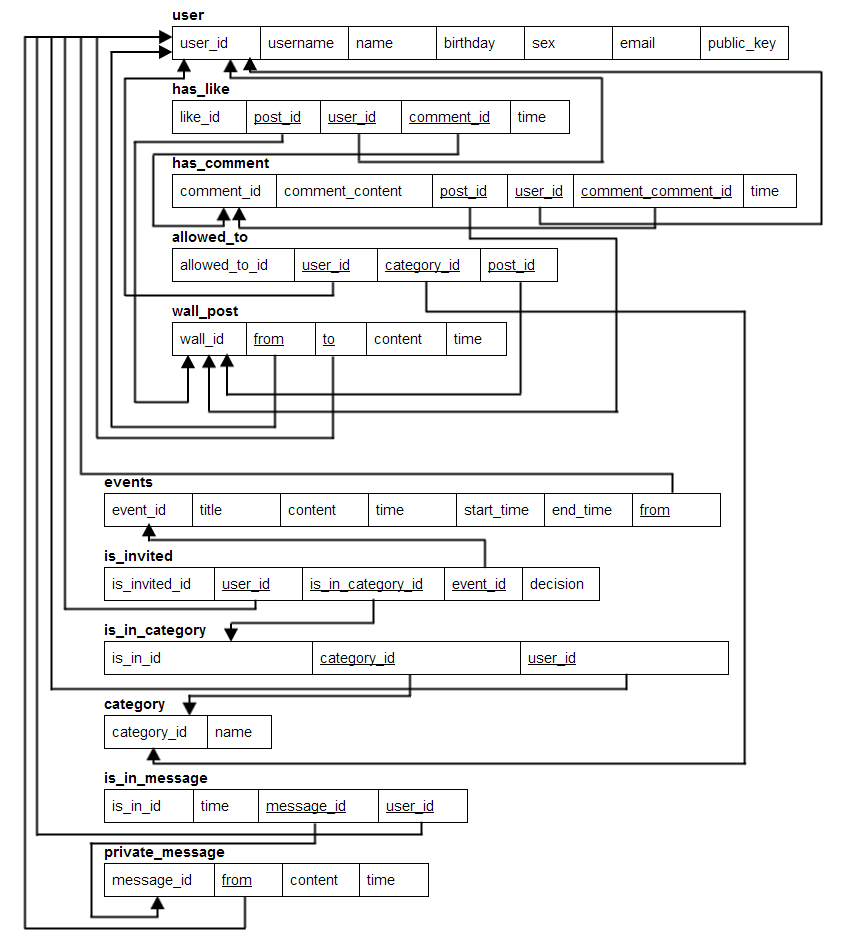
\includegraphics[width=1.4\textwidth]{images/design/logical_diagram.png}
    \caption{Database Entity Relationship diagram}
    \label{fig:db_er_diag}
\end{figure}

\clearpage

\begin{figure}[h]
    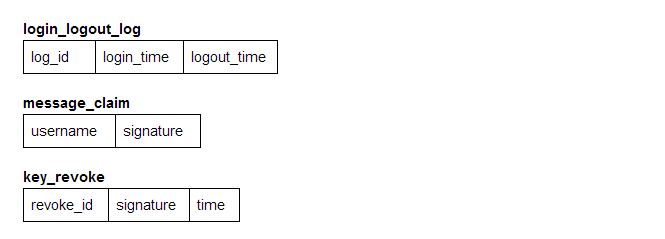
\includegraphics[width=1.4\textwidth]{images/design/logical_diagram2.png}
    \caption{Database Entity Relationship diagram}
    \label{fig:db_er_diag}
\end{figure}

\clearpage

\section{ER Diagram}
\subsection{Database design version 1.0}
\begin{landscape}
\begin{figure}[h]
    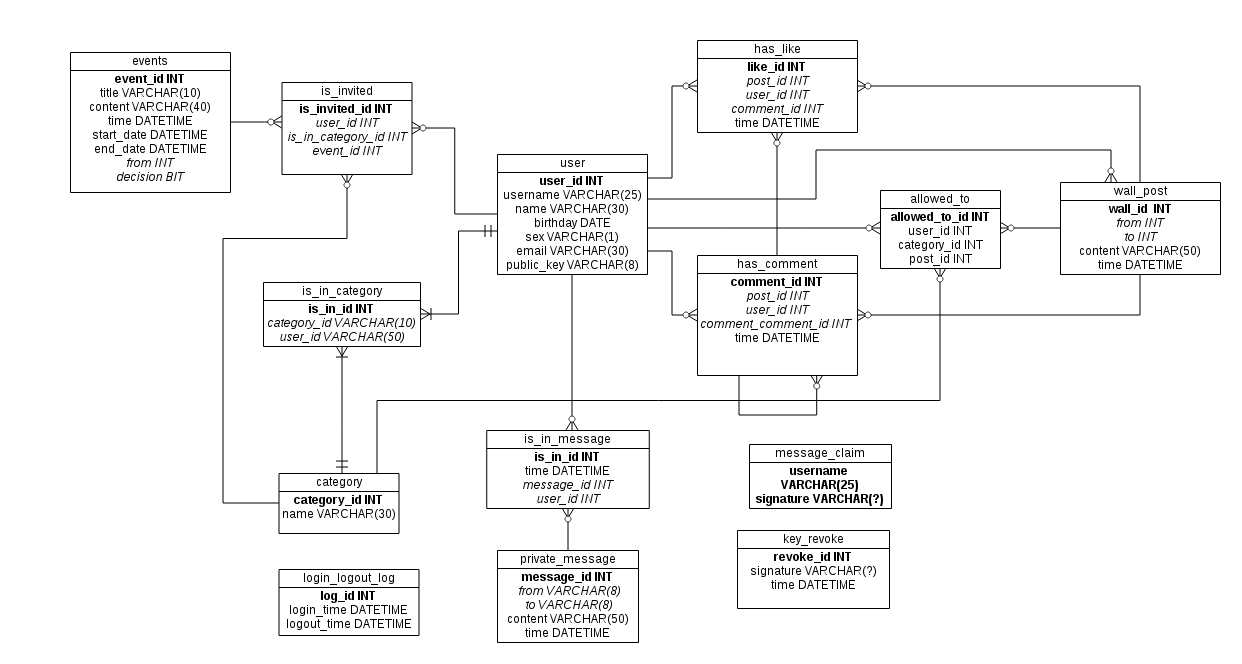
\includegraphics[width=1.4\textwidth]{images/design/project_er_diagram.png}
    \caption{Database Entity Relationship diagram}
    \label{fig:db_er_diag}
\end{figure}
\end{landscape}
